\chapter{Java-Programm}
\label{sec:java-programm}

\section{Anforderungen}
\subsection{Programm}
Die Hauptaufgabe des Programms ist es dem Benutzer eine Möglichkeit zum Steuern der Katzenfütterungsanlage zu Verfügung zu stellen. Weiters soll das Programm die Motoren steuern und die Sensoren in der Anlage auswerten können. Für diese Aufgabe sollen die IO-Pins am Raspberry verwendet werden.
\subsection{Design - Benutzerinterface}
Das Design der GUI-Fenster soll einfach und übersichtlich gestaltet werden. Auf der Hauptseite, also der Seite die immer zu sehen ist, sollen Informationen dargestellt werden, die dem Benutzer einen schnellen Überblick über den Zustand der Anlage geben. Alle anderen nicht direkt ersichtlichen Funktionen sollen über sinnvoll benamte Menüpunkte erreichbar sein.
Der Benutzer soll mit Hilfe eines kleinen Touchdisplays die Möglichkeit haben die Anlage zu steuern. Deswegen muss darauf geachtet werden, dass alle GUI-Fenster sinnvoll per Touch-Gesten verwenbar sind.
\subsection{Externe Steuerung}
Da die Katzenfütterungsanlage die Katze füttern soll, wenn die Familie der Katze auf Urlaub ist, sollte die Anlage auch über das Internet erreichbar sein. Dafür gibt es die Möglichkeit einen Benutzer auf der Anlage anzulegen mit welchem man anschließend über eine Webseite auf die Anlage zugreifen kann. Weiters soll das Java Programm (Server) mit der Web-Applikation (Client) kommunizieren, also Daten austauschen, können.

\newpage

\section{Voruntersuchung}
\subsection{Wieso Java und nicht C?}
Zu Beginn musste entschieden werden mit welcher Programmiersprache gearbeitet werden soll. Zur Auswahl standen Java und C.
Vorteile von C:
\begin{itemize}
\item[1] Echtzeitfähige Steuerung der Motoren und Senosren
\item[2] Hardwarenahe Programmierung für die Pins
\end{itemize}
Vorteile von Java:
\begin{itemize}
\item[1] Erstellen einer GUI ist einfacher
\item[2] Implementieren eines Servers ist einfacher
\end{itemize}

Nach dem Gegenüberstellen der Vorteile wurde Java als Programmiersprache gewählt.

\subsection{Wieso das Raspberry Pi 3 Model B?}
Schon zu Beginn der Diplomarbeit war klar, dass mit deinem Raspberry gearbeitet werden soll. Nun musste entschieden werden welches Model verwendet werden soll. Wir haben das Raspberry Pi 3 Model B aufgrund folgender technischer Daten gewählt:
\begin{itemize}
\item[1] Rechenleistung
\item[2] Anzahl der GPIO-Pins
\item[3] WLAN-Fähigkeit
\end{itemize}

\subsection{Auswahl eines Touchdisplays}
Das Display muss folgendet Anforderungen erfüllen:
\begin{itemize}
\item[1] Es muss ein Touchscreen-Display sein
\item[2] Es muss einfach an das Raspberry anschließbar sein
\item[3] Es sollte nicht zu teuer sein
\end{itemize}

Aufgrund dieser Anforderungen wurde das Touchdisplay von Raspberry gewählt.

\subsection{Wieso pi4j?}
Da Java als Programmiersprache gewählt wurde, musste eine Möglichkeit die GPIO-Pins anzusteuern gefunden werden.
Da bei der Recherche außer pi4j Java kaum etwas gefunden wurde, wurde pi4j gewählt. Weiters vorteilhaft ist, dass das Ansteuern der Pins via Code nicht sehr kopliziert ist. 

\subsection{Wieso Mongodb?}
Eine Datenbank wurde gewählt, weil es gegebüber des Speichers der Daten in eine Datei mehrere Vorteile aufweist. 
\subsubsection{Vorteil gegenüber Daten in Datei speichern}
Vorteile einer Datenbank:
\begin{itemize}
\item[1] Keine Probleme mit Pfaden
\item[2] Daten sind alle in einem Punkt gespeichert und nicht im System verteilt
\item[3] Der benötigte Code für die Datenbank macht das Programm übersichtlicher
\end{itemize}
\subsubsection{Vergleich mit anderen Datenbanken}
Vorteile von Mongodb gegenüber anderen Datenbanken (zB mySQL):
\begin{itemize}
\item[1] Mongodb ist schemenlos (Daten benötigen keine bestimmte Struktur)
\item[2] Mongodb ist kostenfrei
\end{itemize}

\subsection{Kommunikation mit der Web-Applikation}
Der Server mit dem die Web-Applikation kommunizieren kann, wird aufgrund der gewählten Programmiersprache, in Java geschrieben. Der Server wird im Hintergrund aktiv sein und auf Anfragen der Web-Applikation warten. Je nach Anfrage wird der Server Daten zurück senden oder Methoden im Programm aufrufen. Die Daten, die bei der Kommunikation ausgetauscht werden, haben den Datentyp JSON.

\newpage

\section{Umsetzung}
Bei der Umsetzung, also beim Schreiben des Programms, wurde wie folgt vorgegangen. Zuerst wurden alle GUI-Fenster per Hand grob designed. Anschließend wurden diese im Netbeans als JFrame Form erstellt. Genaueres über die GUI-Fenster folgt uner Punkt 2.3.4. Danach wurden grundlegende Funktionen die das Programm zu erfüllen hat implementiert. Weiters wurden noch: Mongodb, pi4j, der Server und der ErrorAndWarningHandler als Singleton implementiert. 
\\ \\ 
Nun folgen ausführlichere Beschreibungen über die oben angeführten Klassen.

\subsection{Mongodb}
\subsubsection{Allgemeines}
Mongodb is ein schemenlose Datenbank. Schemenlos bedeuted, dass die Daten keine besondere Formatierung brauchen um gespeichert zu werden. Zusätzlich wird jedem gespeichertem Datensatz automatisch ein einmaliger Indentifikator gegeben. Weiters ist es kostenfrei und man benötigt keine Lizenzen.
\\
Bei einer schemenbehafteten Datenbank werden die Daten in Reihen und Spalten gegliedert. Um eine solche Datenbank effizient nutzen zu können wird auch ein einmaliger Identifikator.
\\ \\ 
In Mongodb sind Zeilen Collections und Spalten Documents. 
\\ \\
Die Datenbank kann in der Konsole mit dem Befehl \textbf{mongod} gestartet werden. In unserem konkreten Fall am Raspberry startet die Datenbank beim Starten des Raspberry automatisch. Weiters kann in der Konsole mit dem Befehl \textbf{mongo}, sofern die Datenbank gestartet ist, die Mongo-Shell geöffnet werden. In der Shell können alle angelegten Datebanken verwaltet werden. Unter verwalten wird das Ändern, Hinzufügen und Löschen von Daten verstanden. Es können auch neue Datenbanken angelegt oder alte Datenbanken gelöscht werden. 
\\ Befehle:
\begin{itemize}
\item[•] \textbf{show dbs} ... zeigt alle angelegten Datenbanken an
\item[•] \textbf{show collections} ... zeigt alle collections in einer Datebank
\item[•] \textbf{use} ... verwenden einer Datenbank, falls die Datenbank noch nicht existiert wird sie neu erstellt 
\\     (Beispiel: use <Datenbankname>)
\item[•] \textbf{drop()} ... löschen einer Datenbank
\\     (Beispiel: <Datenbankname>.drop() )
\item[•] \textbf{find()} ... suchen nach bestimmten Daten 
\\     (Beispiel: db.data.find() )
\item[•] \textbf{count()} ... zählt die Dokumente in einer Collection
\\     (Beispiel: db.<Collectionname>.count() )
\item[•] \textbf{insert()} ... hinzufügen eines Dokumentes
\\     (Beispiel: db.data.insert(\{"time1":"13:30"\})
\item[•] \textbf{updateOne()} ... updaten von Daten
\\     (Beispiel: db.data.updateOne(<DokumentID>, <Daten>) )
\item[•] \textbf{deleteOne()} ... löschen eins Dokumentes
\\     (Beispiel: db.data.deleteOne(<DokumentID>) )

\end{itemize}

\subsubsection{Datenbankmanagementsystem DBS}
Ein Datenbankmanagementsystem verwaltet eine oder mehrere Datenbanken. Mehrer Datenbanken werden dabei benötigt, wenn mehrere Anwenugen oder Programme jeweils eine eigene Datenbank brauchen. Ein Beispiel für ein DBS ist Mongodb.

\subsubsection{Singleton}
Der Datenbankzugriff wurde in einem Singleton implementiert. Dadurch wird nur ein Objekt der Datenbank erzeugt. Das bedeutet, dass nur von dieser Klasse aus auf die Datenbank zugegriffen wird und nur eine Verbindung geöffnet wird.
\\ Ein weiterer Vorteil davon ist, dass wenn einmal eine andere Datenbank verwendet werden sollte, nur diese eine Klasse geändert werden muss, weil nur in dieser Klasse der Code für die spezifische Datenbank enthalten ist.

\subsubsection{Code Beispiele}
Da am Raspberry die neueste Version von Mongodb nicht funktioniert, wird die Version 2.14.2 verwendet. Weitere Details zu diesem Thema sind unter Punkt 2.4.1 zu finden.
\\ Aus diesem Grund sind auch die Methoden, die als Beispiele angeführt sind, von der älteren Version. 
\\ \\ 
Als erstes muss eine Verbindung mit der Datenbank aufgebaut werden. Falls die Datenbank noch nicht existiert wird sie automatisch erstellt.
Dies ist in Java mit folgenden Methoden möglich:
\begin{lstlisting}[style=JavaStyle]
	MongoClient mongodb = new MongoClient();
	DB database = mongodb.getDB("<Datenbankname>");
\end{lstlisting}

Danach muss die Collection, in der gearbeitet werden soll, ausgewählt werden. Falls die Collection noch nicht existiert wird sie automatisch erstellt. Das ist mit der folgenden Methode möglich:
\begin{lstlisting}[style=JavaStyle]
	DBCollection coll = database.getCollection("<Collectionname>");
\end{lstlisting}
Anschließend kann mit der Datenbank gearbeitet werden. 
\begin{itemize}
\item[•] Die Dokumente in einer Collection zähle1n:
\begin{lstlisting}[style=JavaStyle]
	<Collectionname>.count();
\end{lstlisting}
\item[•] Ein Dokument aus der Datenbank lesen:
\begin{lstlisting}[style=JavaStyle]
	DBObject document = <Collectionname>.find(<Identifikator>).next();
\end{lstlisting}
\item[•] Ein Dokument zu einer Collection hinzufügen:
\begin{lstlisting}[style=JavaStyle]
	<Collectionname>.insert(document);
\end{lstlisting}	
\item[•] Ein Dokument in einer Collection updaten:
\begin{lstlisting}[style=JavaStyle]
	<Collectionname>.update(<Identifikator>, document);
\end{lstlisting}
\end{itemize}

Bevor das Java Programm beendet wird sollte die Verbindung zur Datenbank wie folgt getrennt werden: 
\begin{lstlisting}[style=JavaStyle]
	mongodb.close();
\end{lstlisting}

Ein konkretes Beispiel des Codes aus dem Programm für die Katzenfütterungsanlage sieht so aus:
\begin{lstlisting}[style=JavaStyle]
	DBObject document = collUser.find(
			new BasicDBObject("identifier", "User")).next();
\end{lstlisting}
Diese Zeile Code sucht in der Collection \textbf{collUser} nach dem Dokument mit dem Identifikator \textbf{new BasicDBObject(\grqq{}identifier\grqq{}, \grqq{}User\grqq{})}. Das gefundene Dokument wird dann der Varibale \textbf{document} zugewiesen. 


\subsection{pi4j}
\subsubsection{Allgemeines}
Pi4j ist eine freie Software, welche Bibliotheken zur Verfügung stellt, mit denen es möglich ist, von einem Java Programm, auf die IO-Pins eines Raspberrys zuzugreifen. Dabei kann ein GPIO-Pin als In- oder Ouput definiert werden. Wenn ein Pin als Output definiert wird, kann er den State High (+5V) oder Low (0V) haben. Mit einem Input Pin, können Signale gemessen werden. Das Ergebnis der Messung ist wieder High oder Low. Weiters ist es auch möglich einem Pin einen Listener zuzuweißen. Dieser Listener wartet bis auf diesem Pin ein Event auftritt und führt dann zum Beispiel eine Methode aus. 
\\ \\
Pi4j stellt eine Verbindung von der JVM (Java Virtuaul Machine) zu dem nativen System des Raspberys her. Dadurch wird es möglich von dem Programm auf die Pins zuzugreifen. Die folgende Grafik zeigt welche Bibliotheken dazu verwendetwerden.

\begin{wrapfigure}{l}{0.5\textwidth}
\vspace{-35pt}
  \begin{center}
    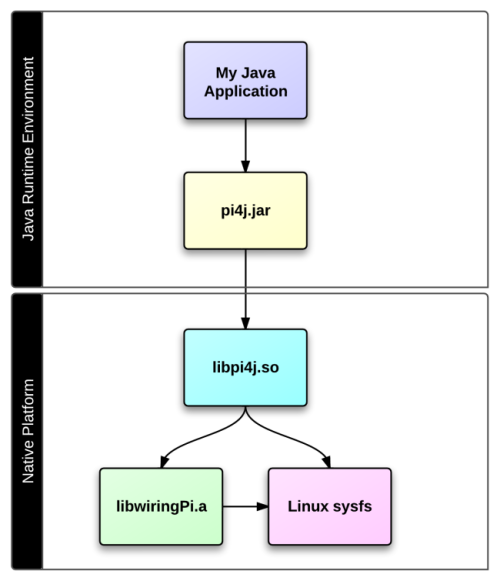
\includegraphics[width=0.45\textwidth]{Bilder/pi4j/dependencies}
  \end{center}
  \caption{Abhängigkeiten}
  \label{Magazin Vorne}
  \vspace{-170pt}
\end{wrapfigure}

Pi4j stellt eine Verbindung von der JVM (Java Virtuaul Machine) zu dem nativen System des Raspberys her. Dadurch wird es möglich von dem Programm auf die Pins zuzugreifen. Die folgende Grafik zeigt welche Bibliotheken dazu verwendetwerden.

\newpage

\subsubsection{Pin Numbering Sheme}

\begin{wrapfigure}{l}{0.5\textwidth}
\vspace{-40pt}
  \begin{center}
    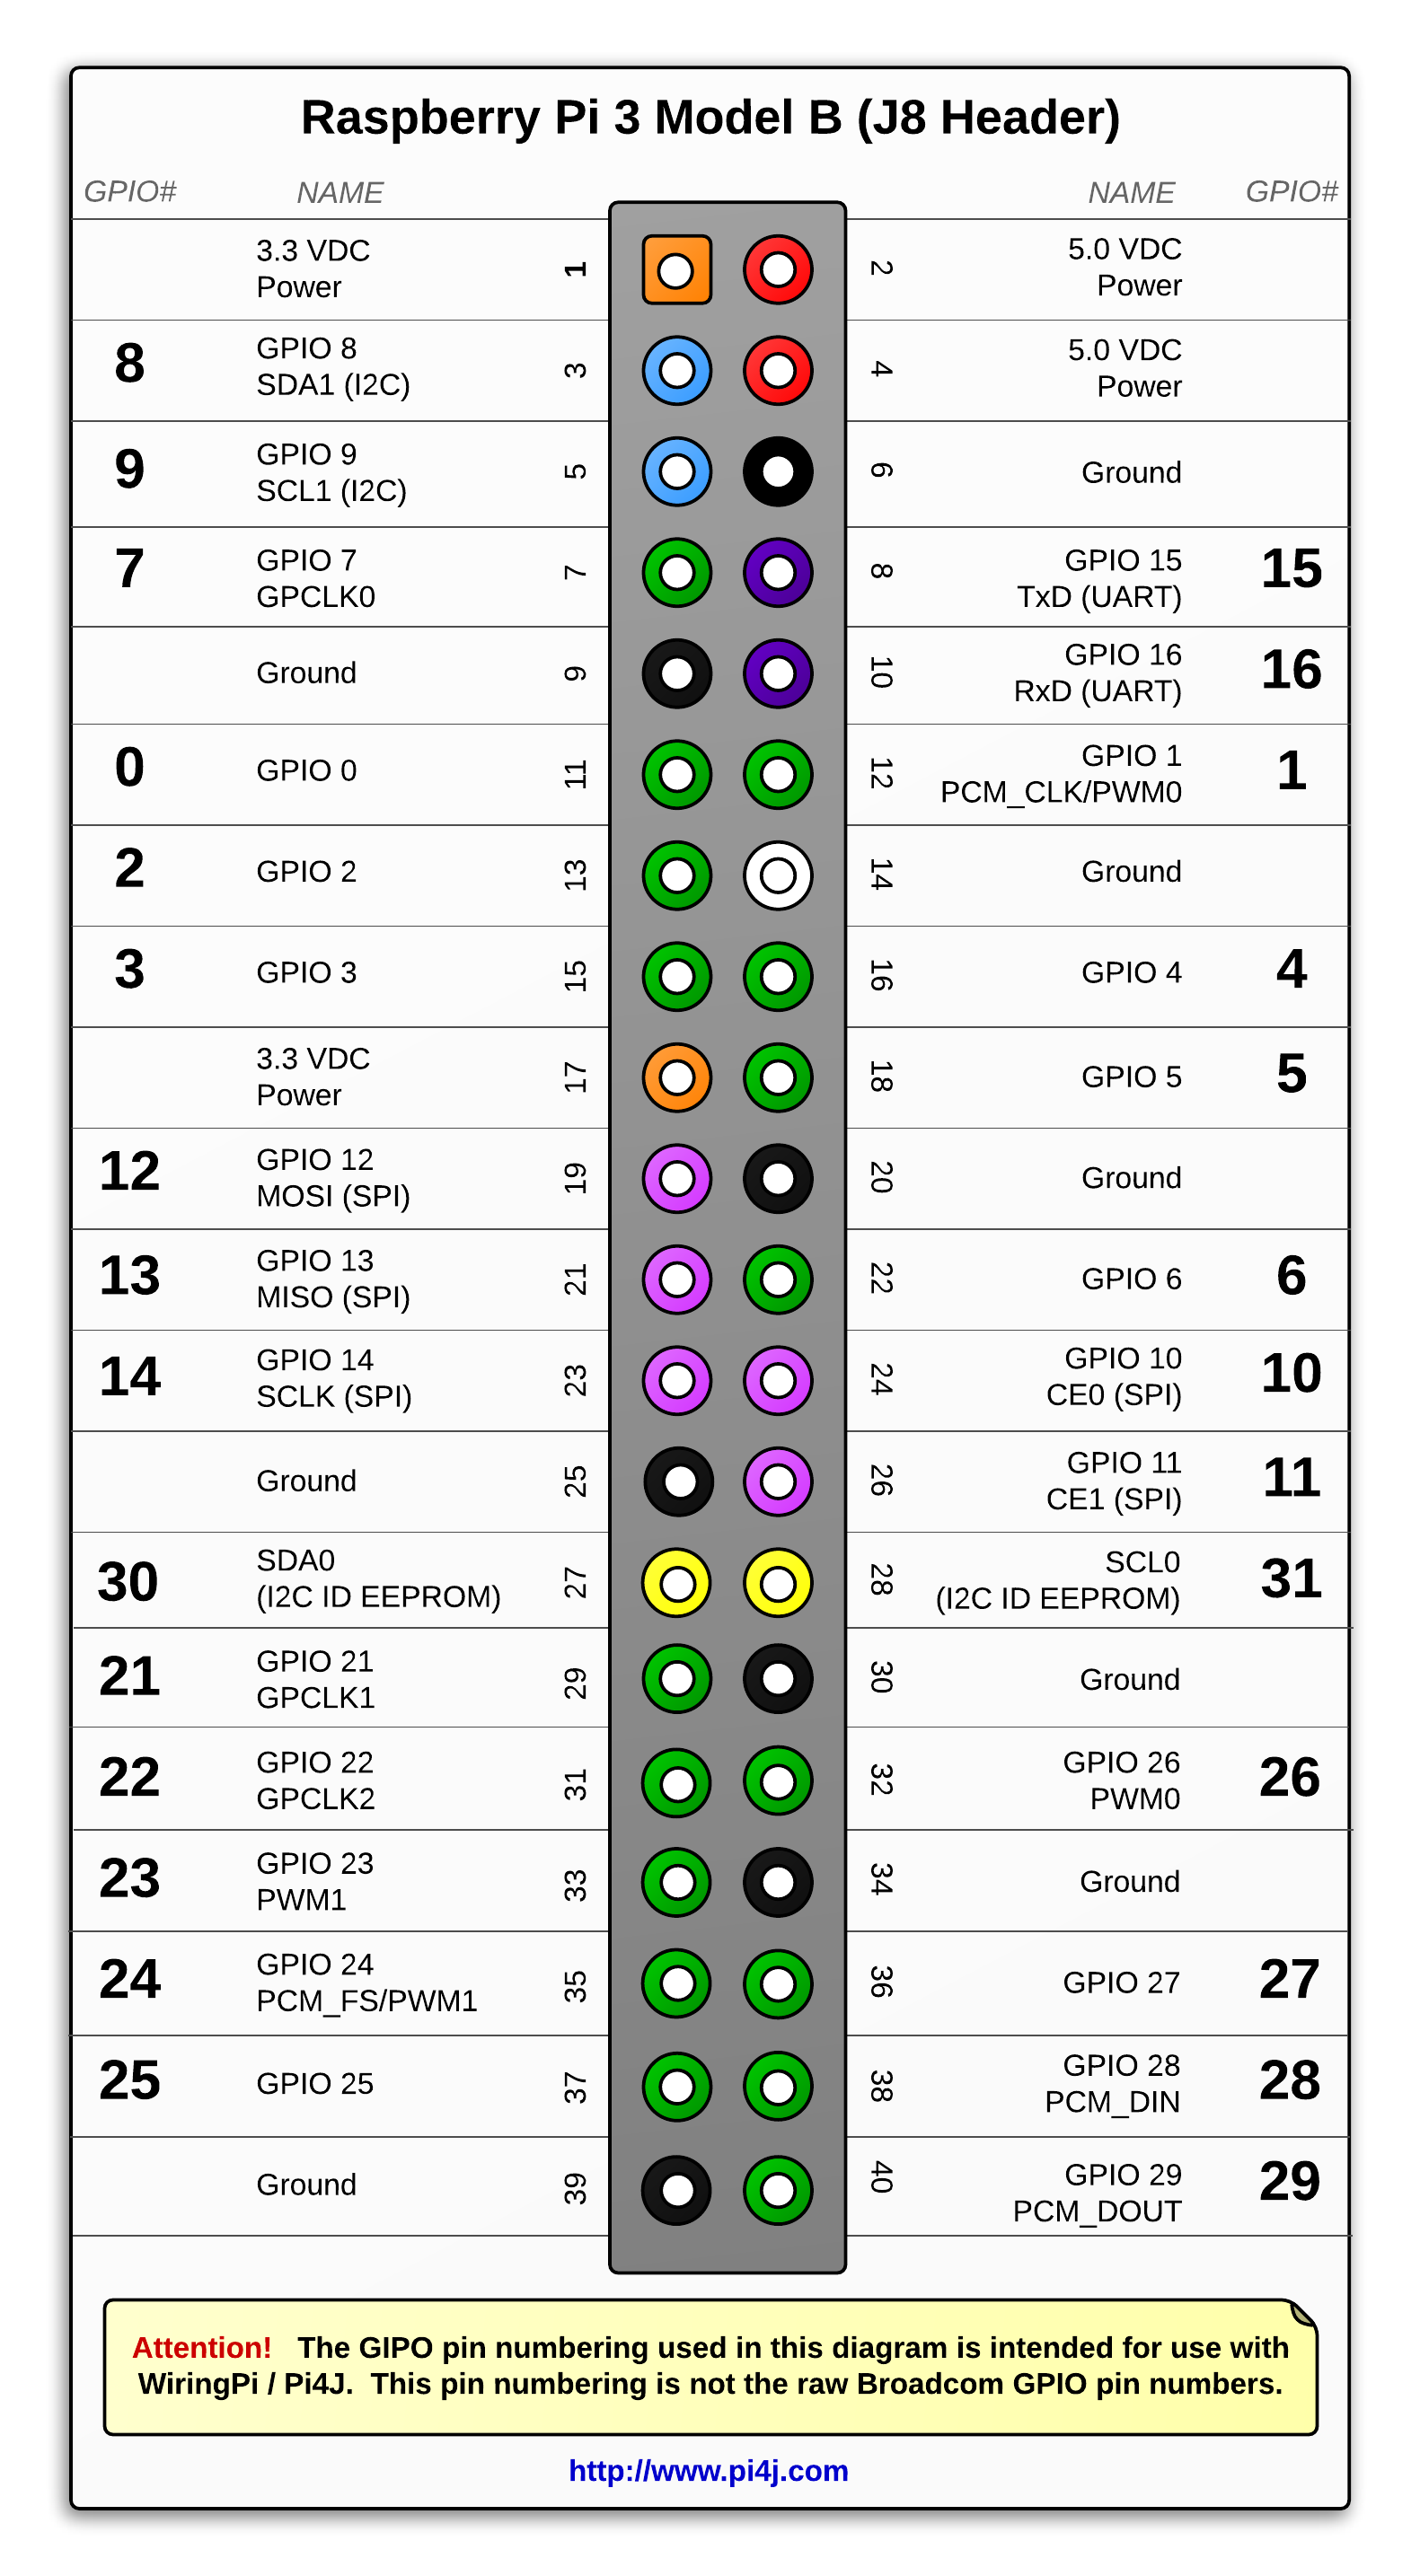
\includegraphics[width=0.50\textwidth]{Bilder/pi4j/PinNumberingSheme}
  \end{center}
  \caption{Pin Numbering Sheme}
  \label{Magazin Vorne}
  \vspace{-320pt}
\end{wrapfigure}

Am Raspberry haben einige Pins schon fest zugewiesene Funktionen, aber bei den GPIO-Pins kann der Programmierer selbst entscheiden, was der Pin sein soll.
\\ \\
In der Grafik ist zu sehen wie die Pins bei einem Raspberry Pi 3 Model B belegt sind.

\vspace{300pt}

\subsubsection{Gewählte Pin Belegung}
Zum Ansteuern der Motoren und Auswerten der Sensoren wurden nur GPIO-Pins verwendet. Die Motoren in der Anlage werden über jeweils eine H-Brücke angesteuert. Das bedeutet, dass jeder der zwei Motoren jeweils mit vier Transitoren angesteuert wird. Jeder Transitor wird von einem eigenen Pin angesteuert. Für die Sensoren wird jeweils ein Pin zum Auswerten benötigt. In Summe werden zehn GPIO-Pins benötigt. 

\newpage

Diese GPIO-Pins werden, wie folgenden Tabelle 2.1 veranschaulicht, verwendet:

\begin{table}[htb]
\centering
\begin{tabular}{|l|l|}
\hline
\textbf{Pin} & \textbf{Verwendungszweck}          \\ \hline
GPIO\_00     & Sensor Schüsselplatte              \\ \hline
GPIO\_01     & Sensor Förderband (Futtersackerl)  \\ \hline
GPIO\_02     & Motor Schüsselplatte: Transistor 1 \\ \hline
GPIO\_03     & Motor Schüsselplatte: Transistor 2 \\ \hline
GPIO\_04     & Motor Schüsselplatte: Transistor 3 \\ \hline
GPIO\_05     & Motor Schüsselplatte: Transistor 4 \\ \hline
GPIO\_06     & Motor Förderband: Transistor 1     \\ \hline
GPIO\_10     & Motor Förderband: Transistor 2     \\ \hline
GPIO\_08     & Motor Förderband: Transistor 3     \\ \hline
GPIO\_09     & Motor Förderband: Transistor 4     \\ \hline
\end{tabular}
\caption{Belegung der GPIO-Pins}
\label{Pinbelegung}
\end{table}

Wenn einer der beiden Sensoren betätigt wird, liefert dieser das Signal High (+5V). Wenn der Sensor nicht betätigt ist liefert dieser Low (0V). 
\\ Um einen Motor einzuschalten müssen jeweils zwei diagonal zueinander liegende Transitoren aktiviert werden. Der Motor dreht sich im Uhrzeigersinn, GPIO-Pins von Transistor 1 und Transistor 4 High sind. Gleichzeitig muss sicher gestellt werden, dass die GPIO-Pins der Transistoren 2 und 3 Low sind. Wenn das nicht sichergestellt ist kann es zu einem Kurzschluss zwischen der Spannungsversorgung und GND kommen. Um den Motor gegen den Uhrzeigersinn zu drehen müssen die GPIO-Pins der Transistoren 2 und 3 auf High sein. 

\subsubsection{Singleton}
Die benötigten Methoden von pi4j wurden in einem Singleton implementiert. Es musste ein Singleton verwendet werden, weil der benötigte Controller für die Pins nur einmal erzeugt werden kann. Wenn der Controller trotzdem öfters erzeugt wird, wird  ein Error geworfen. Der Singleton wird nun dazu verwendet, dass auf die Pins von unterschiedlichen Klassen zugegriffen werden kann. Der Zugriff von mehreren Klassen ist ohne einen Singleton programmiertechnisch nicht lösbar.

\subsubsection{Code Beispiele}
Um mit den GPIO-Pins arbeiten zu können muss zu Beginn ein Controller erstellt werden. Dies ist wie folgt möglich:
\begin{lstlisting}[style=JavaStyle]
	GpioController controller = GpioFactory.getInstance();
\end{lstlisting}
Wenn der Controller erstellt ist kann auf die Pins, mit denen gearbeitet werden soll, zugegriffen werden. Bei einem Pin kann auch eine \textbf{ShutDownOption} angeben werden. Diese gibt an in welchen Zustand der Pin vor dem Herunterfahren gesetzt wird. Dieser Zugriff erfolgt wie folgt: 
\begin{itemize}
\item[•] Zugreigen auf einen Pin als digitalen Input-Pin:
\begin{lstlisting}[style=JavaStyle]
	GpioPinDigitalInput pin = controller.provisionDigitalInputPin(
		RaspiPin.GPIO_00, PinPullResistance.PULL_DOWN);
	pin.setShutdownOptions(true);
\end{lstlisting}
\item[•] Zugreigen auf einen Pin als digitalen Output-Pin:
\begin{lstlisting}[style=JavaStyle]
	GpioPinDigitalOutput pin = controller.provisionDigitalOutputPin(
		RaspiPin.GPIO_02, PinState.LOW);
	pin.setShutdownOptions(true, PinState.LOW);
\end{lstlisting}
\end{itemize}
Wenn das erledigt ist kann mit dem Pin gearbeitet werden. Dies kann wie in den folgenden Beispielen erfolgen:
\begin{itemize}
\item[•] Zustand eines Input-Pins auswerten: 
\begin{lstlisting}[style=JavaStyle]
	pin.getState()
\end{lstlisting}
Diese Methode liefert den Zustand des Pins zurück. Dieser kann High oder Low sein.
\item[•] Zustand eines Output-Pins setzen:
\begin{lstlisting}[style=JavaStyle]
	pin.low();	
	pin.high();
\end{lstlisting}
Mit \textbf{pin.low()} kann der Zustand eines Pins auf Low (0V) und mit \textbf{pin.high()} auf High (+5V) gesetzt werden. 
\end{itemize}

Vor dem Beenden des Java Programmes sollte der Controller wie folgt heruntergefahren werden:
\begin{lstlisting}[style=JavaStyle]
	controller.shutdown();
\end{lstlisting}

\newpage

\subsection{Server-Client-Kommunikation}
\subsubsection{Server}
Der Server wird beim Starten des Java Programmes in einem eigenen Thread gestartet. In diesem Thread wartet der Server bis ein Client versucht Kontakt mit ihm aufzunehmen. Wenn die Verbindung akzeptiert wird, wird ein neuer Thread geöffnet in dem die Kommunikation mit diesem Client abläuft. Sobald die Kommunikation beendet ist wird der Thread wieder geschlossen. 
\\ Der Server wurde auch als Singleton implementiert damit von mehreren Klassen ausgehend auf ihn zugegriffen werden kann.

\subsubsection{Übertragungsprotokoll}
Im Übertragungsprotokoll wird festgelegt wie die Kommunikation zwischen Server und Client abläuft. Hier wird festgelegt was ein gültige Request (Anfrage) ist und wie die Response (Antwort) auf den jeweiligen Request aussieht. 
\\ \\
Wenn der Request des Clients mit einem \textbf{GET} beginnt, bedeutet dass, das der Client Daten vom Server fordert. Beginnt der Request mit einem \textbf{PUT}, bedeutet dass, das der Client dem Server Daten schicken will.
\\ Nach jedem \textbf{GET} oder \textbf{PUT} folgt ein URL der angibt, welche Daten der Client fordert oder welche Daten der Client dem Server schicken will.
\\ \\
Die folgende Tabelle zeigt alle gültigen Requests und die jeweilige Response darauf:

\begin{table}[htb]
\centering
\begin{tabular}{|l|l|p{300pt}|}
\hline
\multicolumn{2}{|c|}{\textbf{Request}}                                    & \multicolumn{1}{c|}{\multirow{2}{*}{\textbf{Response}}}                                          \\ \cline{1-2}
\multicolumn{1}{|c|}{\textbf{Aktion}} & \multicolumn{1}{c|}{\textbf{URL}} & \multicolumn{1}{c|}{}                                                                            \\ \hline
GET                                   & /errors\_warnings                 & Der Server schickt dem Client die aktuell anzuzeigenden Errors und Warnungen in einer Json-Array \\ \hline
PUT                                   & /ChangeMachineState               & Der Server ruft eine Methode auf um den Maschinenzustand zu ändern                               \\ \hline
\end{tabular}
\caption{Übertragungsprotokoll}
\label{Übertragungsprotokoll}
\end{table}

\newpage

\subsubsection{Response-GET}
Wenn der Server einen Request mit dem Beginn \textbf{GET} bekommt, muss er dem Client die Daten schicken. 
\\ Bei der Katzenfütterungsanlage werden dem Client vom Server die ganzen auftretenten Errors und Warnungen geschickt. Die Errors und Warnungen werdem dem Client als Json-Array geschickt. Diese Json-Array wird in der Klasse, welche alle Errors and Warnungen verarbeitet, erstellt. Die Json-Array ist unter Punkt \ref{subsubsec:Array} dargestellt. 

\subsubsection{Response-PUT}
Wenn der Server einen Request mit dem Beginn \textbf{PUT} bekommt, muss er Daten vom Client entgegen nehmen.
\\ Bei der Katzenfütterungsanlage bekommt der Server die Daten nicht direkt. Da der Maschinenzustand nur \textbf{Ein} oder \textbf{Aus} sein kann, wird dieser nicht übermittelt. Stattdessen wird, wenn der Maschinenzustand geändert wird, die Methode \textbf{machineStateChanger()} aufgerufen, welche ihn ändert. Diese Methode aktualisiert auch die GUI-Elemente am Raspberry, abhägig vom Maschinenzustand. 

\subsection{Errors und Warnungsverarbeitung}
\subsubsection{Allgemeines}
Der Benutzer der Katzenfütterungsanlage muss über Fehler, die während des Programmablaufs auftreten, informiert werden. 
\\ Dazu dient die \textbf{ErrorAndWarningHandler\_Singleton} Klasse. In dieser Klasse wird beim Auftreten eines Fehlers eine Boolean Variable auf \textbf{true} gesetzt. Beim Erstellen der Liste, die die Errors und Warnungen enthält, werden die jeweiligen Boolean-Variablen abgefragt. Wenn die Boolean-Variable \textbf{true} ist, wird der Error oder die Warnung hinzugefügt. 

\newpage

\subsubsection{Errors und Warnungen aktivieren/deaktivieren}
Um die Boolean-Variable, die die Errors and Warnungen aktiviert, auf true zu setzen, muss die jeweils zum Error oder zur Warnung gehörende Methode aufgerufen werden. Diese Methode kann wie folgt aussehen:
\begin{lstlisting}[style=JavaStyle]
public void setFeedingHasFailedError (Boolean errorOn, String errorTime)
    {
        error_hasFeedingFailed = errorOn;
        failedFeedingTime = errorTime;
    }
\end{lstlisting}
In diesem konkreten Beispiel wird der Error, der dem Benutzer mitteilt, dass eine Fütterung fehlgeschlagen hat, aktiviert. Mit dem Parameter \textbf{errorOn} kann bestimmt werden, ob der Error aktiv oder inaktiv sein soll. Wenn der Parameter \textbf{true} ist, ist der Error aktiv. Daraus folgt, dass der Error inaktiv ist, wenn \textbf{errorOn = false} ist. 
\\ Mit dem zweiten Parameter \textbf{errorTime} wird die Zeit übergeben, zu der die Fütterung fehlgeschlagen ist. Diese Zeit wird dann in der Errormeldung ausgegeben. 

\subsubsection{Json-Array} \label{subsubsec:Array}
Diese Klasse stellt auch die Json-Array zur Verfügung, welche dann dem Client (Web-Applikation) geschickt wird. 

Die JsonArray sieht wie folgt aus:

\begin{lstlisting}[language=json,firstnumber=1]
{ 
	"Errors": 
	[ 
		{"message" : "Error1", "hidden" : false}, 
		{"message" : "Error2", "hidden" : false} 
	] 
	"Warnings": 
	[ 
		{"message" : "Warning1", "hidden" : false}, 
		{"message" : "Warnung2", "hidden" : false} 
	] 
} 
\end{lstlisting}

\newpage

\subsubsection{Listenmodel}
Die Zeile, in der die Klasse für das Listenmodel angelegt wird, sieht wie folgt aus:
\begin{lstlisting}[style=JavaStyle]
	public class ErrorAndWarningModel extends AbstractListModel
\end{lstlisting}
Nach dem Klassennamen muss \textbf{extends AbstractListModel} hinzugefügt werden. Dies bedeutet, dass das erstellte Listemodel eine Vererbung von \textbf{AbstractListModel} ist.
\\ \\
Das Listenmodel wird wie folgt angelegt:
\begin{lstlisting}[style=JavaStyle]
	private final List<String> errorAndWarning;
\end{lstlisting}
Damit ist nun festgelegt, dass die Elemente in der Liste Strings sind. 

\subsubsection{Liste}
Eine Liste in Java wird dazu verwendet, um mehrere Daten in einem Objekt zu speichern. Die Liste kann wie folgt erstellt werden:
\begin{lstlisting}[style=JavaStyle]
	List<String> list = new ArrayList();
\end{lstlisting}
Das Objekt der Liste verfügt über eigene Methoden. 
\begin{itemize}
\item[•] Anzahl der Elemente in der Liste zählen: 
\begin{lstlisting}[style=JavaStyle]
	list.size();
\end{lstlisting}
\item[•] Hinzufügen eines Elementes:
\begin{lstlisting}[style=JavaStyle]
	list.add("Das ist ein Element!");
\end{lstlisting}
\item[•] Leeren der Liste (Löschen aller Elemente)
\begin{lstlisting}[style=JavaStyle]
	list.clear();
\end{lstlisting}
\end{itemize}

Die Errors und Warnungen, die in der Liste gespeichert werden, werden in der GUI in einer Liste (jList) dargestellt. Siehe Kapitel \ref{subsubsec:MainWindow}. 

\subsection{SwingWorker}
Der SwingWorker in Java wird benötigt, wenn eine Anwendung mehr Zeit benötigt. Mithilfe des SwingWorkers kann diese Aktion im Hintergrund ausgeführt werden. Der Vorteil davon ist, dass die GUI verwendbar bleibt und nicht blockiert. Dafür wird dann mit Hilfe des SwingWorkers ein Hintergrund-Thread geöffnet in dem die Aktion, die mehr Zeit benötigt, abgearbeitet wird.
\\ \\ Um den SwingWorker verwenden zu können, muss die Klasse wie folgt erstellt werden:
\begin{lstlisting}[style=JavaStyle]
private class TimeOfDayAndDateWorker extends SwingWorker<Object, String>
\end{lstlisting}
Im Generic steht als erstes der Rückgabewert von \textbf{done()} und als zweites der Rückgabewert von \textbf{process()}.

\subsubsection{EDT}
Im Event Dispatch Thread (EDT) wird die GUI sequentiell abgearbeitet. Dies bedeutet, dass alle Methoden ihre benötigte Zeit in Anspruch nehmen und danach die jeweils Nächste ausgeführt wird. Im Grunde wird dann ein SwingWorker verwendet, wenn die GUI für den Benutzer merklich blockiert. 

\subsubsection{Methoden des SwingWorkers}
\begin{itemize}
\item[•] doInBackground()
\item[•] done()
\item[•] process()
\end{itemize}

\subsection{GUI-Fenster}
\subsubsection{MainWindow} \caption{subsubsec:MainWindow}
\subsubsection{TimeManagement}
\subsubsection{CreateUser}
\subsubsection{ManualControl}
\subsubsection{Positionsinformation}
\subsubsection{SystemInfo}
\subsubsection{Update}

\section{Zusammenfassung/Verbesserungsmöglichkeiten}
\subsection{Probleme mit Mongodb am Raspberry}
\subsection{Probleme mit pi4j -> Snapshotversion verwendet - ansonsten werden pins nicht erkannt}
\subsection{GUI auf "Touchscreen-Design" abändern}
\subsection{Besser Benutzerverwaltung - Mehrere Benutzer anlegen}
\subsection{Selbst erstellbare Vorlagen in denen Zeiten gespeichert werden}
